\chapter{الكربونيلات المترافقة: مايكل وروبنسون}\label{ch:b2:conjugate-additions}

جُمعت الحلقات الأربع لهرمون ستيرويدي أول مرة حلقةً حلقة، وصارت سلسلة واحدة من
التفاعلات الطريقة المعيارية لإضافة حلقة: فهي تبني حلقة سداسية كاملة، بكيتونها،
من كيتون وكيتون صغير غير مشبع. وهي تنجح لأن مجموعة الكربونيل المترافقة
مع رابطة مزدوجة \ce{C=C} تنقل طابعها المحب للإلكترونات إلى الطرف البعيد من تلك الرابطة المزدوجة.
وهذا الفصل يدور حول ذلك الطرف البعيد: أي المحبات للنواة تهاجمه، ولماذا، وما الذي يمكن بناؤه به.

\begin{recall}
\Cref{ch:b2:enolates-aldol}: أيونات الإينولات، \omterm{def:b2:enolates-aldol:aldol}{والتكاثف الألدولي}. و\cref{ch:b2:frontier-orbitals}: \omterm{def:b2:frontier-orbitals:control}{التحكم
بالشحنة} \omterm{def:b2:frontier-orbitals:control}{والتحكم المداري}، والكواشف القاسية واللينة. و\cref{ch:b2:huckel}: مدارات هوكل وشحنات $\pi$.
ومجلد السنة الأولى: كواشف غرينيار والهيدريدات، والتحكم الحركي والترموديناميكي، والأنظمة
المترافقة.
\end{recall}

\section{موقعان محبان للإلكترونات}

\begin{definition}[المركبات الكربونيلية $\alpha,\beta$-غير المشبعة]\label{def:b2:conjugate-additions:enone}
\emph{المركب الكربونيلي $\alpha,\beta$-غير المشبع}\index{مركب كربونيلي ألفا،بيتا-غير مشبع@مركب كربونيلي $\alpha,\beta$-غير مشبع}
له رابطة مزدوجة \ce{C=C} بين الكربونين $\alpha$
و$\beta$ لمركب كربونيلي، مترافقة مع \ce{C=O}: إينون (كيتون)، أو إينال
(ألدهيد)، أو إستر أو \omterm{def:b2:amines:nitrile}{نتريل} غير مشبع. وأبسطها البروبينال \ce{CH2=CHCHO} 
والبوت-3-ين-2-ون \ce{CH2=CHCOCH3} (ميثيل فينيل كيتون).
\end{definition}

\begin{omfigure}
\setchemfig{atom sep=1.9em}
\schemestart
\chemfig{H_2C=CH-CH=O}
\arrow{<->}
\chemfig{H_2C=CH-\chemabove{C}{\scriptstyle +}H-\chemabove{O}{\scriptstyle -}}
\arrow{<->}
\chemfig{\chemabove{C}{\scriptstyle +}H_2-CH=CH-\chemabove{O}{\scriptstyle -}}
\schemestop
\par\medskip

\begin{tikzpicture}
\begin{axis}[ybar, width=0.47\linewidth, height=4.6cm, ymin=-0.6, ymax=0.4,
  xtick={1,2,3,4}, xticklabels={C$\beta$,C$\alpha$,C(O),O}, axis x line=bottom, axis y line=left,
  extra y ticks={0}, extra y tick style={grid=major, grid style={black!50}}, enlarge x limits=0.15,
  tick label style={font=\scriptsize}, ylabel={\foreignlanguage{arabic}{شحنة $\pi$}}, label style={font=\small},
  title={\small \foreignlanguage{arabic}{شحنات $\pi$ في البروبينال}}, bar width=8pt]
\addplot[fill=omDef!50, draw=omDef] table[x=atom, y=q] {figdata/out/bachelor-2-huckel-d.dat};
\end{axis}
\end{tikzpicture}\hfill
\begin{tikzpicture}
\begin{axis}[ybar, width=0.47\linewidth, height=4.6cm, ymin=-0.8, ymax=0.8,
  xtick={1,2,3,4}, xticklabels={C$\beta$,C$\alpha$,C(O),O}, axis x line=bottom, axis y line=left,
  extra y ticks={0}, extra y tick style={grid=major, grid style={black!50}}, enlarge x limits=0.15,
  tick label style={font=\scriptsize}, ylabel={\foreignlanguage{arabic}{المعامل}}, label style={font=\small},
  title={\small \foreignlanguage{arabic}{مدار \babelsublr{LUMO} في البروبينال}}, bar width=8pt]
\addplot[fill=omThm!45, draw=omThm] table[x=atom, y=c] {figdata/out/bachelor-2-huckel-d.dat};
\end{axis}
\end{tikzpicture}

{\small البروبينال. في الأعلى: بنى رنينه الثلاث؛ وتضع الأخيرتان شحنة موجبة على
كربون الكربونيل وعلى الكربون $\beta$. وفي الأسفل: نموذج هوكل في
\cref{ch:b2:frontier-orbitals} ($\alpha_{\ce{O}} = \alpha + \beta$، $\beta_{\ce{CO}} = \beta$؛ وهو نموذج).
أكبر شحنة موجبة على كربون الكربونيل (+0.33، مقابل +0.23 على الكربون $\beta$)؛ 
وأكبر معامل في المدار \omterm{def:b2:frontier-orbitals:frontier}{LUMO} على الكربون $\beta$ (0.66، مقابل $-0.58$).}
\end{omfigure}

\begin{proposition}[موقعان]\label{prop:b2:conjugate-additions:two-sites}
في المركب الكربونيلي $\alpha,\beta$-غير المشبع، يكون كربون الكربونيل والكربون $\beta$ كلاهما
محبًا للإلكترونات. ويحمل كربون الكربونيل الشحنة الموجبة الأكبر؛ ويحمل الكربون $\beta$ المعامل
الأكبر في المدار \omterm{def:b2:frontier-orbitals:frontier}{LUMO}.
\end{proposition}

\begin{proof}[تعليل]
تضع بنى الرنين شحنة موجبة على كربون الكربونيل، وعبر \ce{C=C}، على
الكربون $\beta$؛ ولا يكون الكربون $\alpha$ موجبًا أبدًا. ونموذج هوكل للبروبينال يجعل ذلك
كميًا: فجمع $2c^2$ على المدارين $\pi$ المشغولين يعطي شحنات $\pi$
(\cref{def:b2:huckel:indices}) $+0.33$ على كربون الكربونيل، و$+0.23$ على الكربون $\beta$، و$-0.03$
على الكربون $\alpha$ و$-0.53$ على الأكسجين. والمدار \omterm{def:b2:frontier-orbitals:frontier}{LUMO}، الذي يستقبل إلكترونات المحب للنواة،
أكبر ما يكون عند الكربون $\beta$. فيستجيب الموقعان إذن لنوعي التحكم
في \cref{def:b2:frontier-orbitals:control}.
% figdata: bachelor-2/huckel.py part d
\end{proof}

\section{إضافة 1،2 أم إضافة مترافقة}

\begin{definition}[أنماط الإضافة]\label{def:b2:conjugate-additions:addition-modes}
المحب للنواة الذي يُضاف إلى كربون الكربونيل في مركب كربونيلي $\alpha,\beta$-غير مشبع يعطي
\emph{إضافة 1،2}\index{إضافة 1،2} (عدًّا من الأكسجين): ألكوكسيدًا أليليًا، ثم
كحولًا. والمحب للنواة الذي يُضاف إلى الكربون $\beta$ يعطي \emph{إضافة مترافقة}\index{إضافة مترافقة}
(أو إضافة 1،4): أيون إينولات، يُبرتن على الكربون فيعطي مركبًا كربونيليًا مشبعًا
مستبدلًا عند الكربون $\beta$.
\end{definition}

\begin{omfigure}
\setchemfig{atom sep=1.9em}
\schemestart
\chemfig{*6(-=-(=O)---)}
\arrow{->[\ce{CH3Li}][ثم \ce{H2O}]}[,1.4]
\chemfig{*6(-=-(-[:75]CH_3)(-[:-15]OH)---)}
\schemestop
\hspace{2.5em}
\schemestart
\chemfig{*6(-=-(=O)---)}
\arrow{->[\ce{(CH3)2CuLi}][ثم \ce{H2O}]}[,1.6]
\chemfig{*6(-(-CH_3)--(=O)---)}
\schemestop
\par\vspace{6pt}

{\small الهكس-2-ين حلقي-1-ون مع محبين للنواة ميثيليين. ميثيل الليثيوم، وهو \omterm{def:b2:frontier-orbitals:hard-soft}{محب للنواة قاسٍ}، يُضاف إلى
كربون الكربونيل: 1-ميثيل هكس-2-ين حلقي-1-ول (\omterm{def:b2:conjugate-additions:addition-modes}{إضافة 1،2}). وثنائي ميثيل كوبرات الليثيوم، وهو محب لين،
يُضاف إلى الكربون $\beta$: 3-ميثيل هكسانون حلقي (\omterm{def:b2:conjugate-additions:addition-modes}{إضافة مترافقة}).}
\end{omfigure}

\begin{proposition}[أي موقع]\label{prop:b2:conjugate-additions:regio}
\omterm{def:b2:frontier-orbitals:hard-soft}{المحبات للنواة القاسية} (المركبات العضوية الليثيومية، ومعظم كواشف غرينيار، و\ce{LiAlH4}) تُضاف أساسًا \omterm{def:b2:conjugate-additions:addition-modes}{إضافة 1،2}، تحت \omterm{def:b2:frontier-orbitals:control}{التحكم
بالشحنة}، وعادة على نحو غير عكوس. \omterm{def:b2:frontier-orbitals:hard-soft}{والمحبات للنواة اللينة} (\omterm{def:b2:conjugate-additions:cuprate}{الكوبرات العضوية}، وأيونات الإينولات المثبتة، والثيولات،
والأمينات) تُضاف أساسًا إضافة 1،4، تحت \omterm{def:b2:frontier-orbitals:control}{التحكم المداري}؛ وناتج \omterm{def:b2:conjugate-additions:addition-modes}{الإضافة المترافقة}، الذي يحتفظ بالرابطة \ce{C=O}، هو
أيضًا الناتج الأكثر استقرارًا.
\end{proposition}

\begin{proof}[تعليل]
\omterm{def:b2:frontier-orbitals:hard-soft}{المحب للنواة القاسي}، الصغير والمشحون، يتآثر أساسًا عبر الشحنات: فيذهب إلى المركز الأكثر
إيجابية، كربون الكربونيل (\cref{prop:b2:conjugate-additions:two-sites})؛ وإضافته سريعة 
ولا تنعكس، فيبقى ناتج 1،2، المتكوّن أسرع (تحكم حركي). أما \omterm{def:b2:frontier-orbitals:hard-soft}{المحب للنواة اللين}،
الكبير والقابل للاستقطاب، ذو المدار \omterm{def:b2:frontier-orbitals:frontier}{HOMO} المرتفع، فيتآثر أساسًا عبر \omterm{def:b2:frontier-orbitals:frontier}{المدارات الحدودية}: فيذهب حيث
يكون المدار \omterm{def:b2:frontier-orbitals:frontier}{LUMO} أكبر، أي الكربون $\beta$. وناتج 1،4 يحتفظ برابطة $\pi$ في \ce{C=O}، أقوى من
رابطة $\pi$ في \ce{C=C} التي يحتفظ بها ناتج 1،2؛ وحين تكون الإضافات عكوسة (السيانيد، والأمينات،
وأيونات الإينولات المثبتة، والألكوكسيدات)، ينجرف التوازن إذن نحو ناتج \omterm{def:b2:conjugate-additions:addition-modes}{الإضافة المترافقة} حتى لو تكوّن
ناتج 1،2 أولًا (تحكم ترموديناميكي).
\end{proof}

\begin{method}[التنبؤ بنمط الإضافة]\label{met:b2:conjugate-additions:predict-mode}
\begin{enumerate}
  \item صنّف المحب للنواة: قاسٍ (\ce{RLi}، \ce{RMgX}، \ce{LiAlH4}، \ce{NaBH4} مع ألدهيد)
        أو لين (\ce{R2CuLi}، أيون إينولات 1،3-ثنائي الكربونيل، \ce{RS-}، \ce{R2NH}، السيانيد عند التوازن).
  \item تحقق من العكوسية: الإضافة القاسية غير العكوسة تعطي ناتج 1،2؛ والعكوسة تعطي،
        إذا أُعطيت الوقت، ناتج 1،4.
  \item تحقق من الإعاقة: الكربون $\beta$ المستبدَل يبطئ الإضافة 1،4؛ والألدهيد، الأقل إعاقة
        والأكثر تفاعلية عند كربونيله من الكيتون، يحابي 1،2.
  \item اكتب \omterm{def:b2:enolates-aldol:enolate}{أيون الإينولات} المتكوّن بالإضافة 1،4: يمكن برتنته، أو احتجازه بمحب
        للإلكترونات.
\end{enumerate}
\end{method}

\section{إضافات مايكل}

\begin{definition}[إضافة مايكل]\label{def:b2:conjugate-additions:michael}
\emph{إضافة مايكل}\index{إضافة مايكل} هي \omterm{def:b2:conjugate-additions:addition-modes}{الإضافة المترافقة} لأنيون كربوني مثبَّت،
عادة أيون إينولات، إلى مركب كربونيلي $\alpha,\beta$-غير مشبع أو ألكين مماثل فقير
بالإلكترونات. والمحب للنواة هو \emph{مانح مايكل}\index{مانح مايكل} (مركب 1،3-ثنائي الكربونيل، أو
نترو ألكان، أو سيانو إستر)؛ والمركب غير المشبع هو \emph{مستقبل مايكل}\index{مستقبل مايكل}
(إينون، أو إينال، أو إستر أو \omterm{def:b2:amines:nitrile}{نتريل} أو مركب نترو غير مشبع).
\end{definition}

\begin{omfigure}
\setchemfig{atom sep=1.8em}
\schemestart
\chemfig{CH_2(-[:30]COOEt)(-[:-30]COOEt)}
\arrow{<=>[\ce{EtO-}][$-$ \ce{EtOH}]}[,1.3]
\chemfig{\chemabove{C}{\scriptstyle -}H(-[:30]COOEt)(-[:-30]COOEt)}
\+
\chemfig{H_2C=CH-C(=[2]O)-CH_3}
\schemestop

\medskip
\setchemfig{atom sep=1.6em}
\schemestart
\arrow{->[إضافة]}[,0.95]
\chemfig{CH(-[:150]EtOOC)(-[:210]EtOOC)-CH_2-CH=C(-[2]\chemabove{O}{\scriptstyle -})-CH_3}
\arrow{->[\ce{EtOH}][$-$ \ce{EtO-}]}[,1.1]
\chemfig{CH(-[:150]EtOOC)(-[:210]EtOOC)-CH_2-CH_2-C(=[2]O)-CH_3}
\schemestop
\par\vspace{6pt}

{\small \omterm{def:b2:conjugate-additions:michael}{إضافة مايكل} لبروبانديوات ثنائي الإيثيل إلى البوت-3-ين-2-ون. يكوّن الإيثوكسيد \omterm{def:b2:enolates-aldol:enolate}{أيون الإينولات}
المثبت؛ فيُضاف إلى الكربون $\beta$؛ ويأخذ \omterm{def:b2:enolates-aldol:enolate}{أيون الإينولات} المتكوّن بروتونًا من الإيثانول، مما
يجدد الإيثوكسيد. والناتج، (3-أوكسوبيوتيل)بروبانديوات ثنائي الإيثيل، مركب 1،5-ثنائي
الكربونيل.}
\end{omfigure}

\begin{proposition}[آلية مايكل]\label{prop:b2:conjugate-additions:michael}
تجري \omterm{def:b2:conjugate-additions:michael}{إضافة مايكل} في ثلاث خطوات (نزع بروتون المانح، \omterm{def:b2:conjugate-additions:addition-modes}{والإضافة المترافقة}، وبرتنة
\omterm{def:b2:enolates-aldol:enolate}{أيون الإينولات} الجديد)، وتتجدد القاعدة في الخطوة الأخيرة: فتكفي كمية حفزية منها.
\end{proposition}

\begin{proof}[تعليل]
هيدروجين $\alpha$ في المانح، الواقع بين كربونيلين، حمضي: $\mathrm pK_a$ نحو 13 لبروبانديوات
ثنائي الإيثيل، و10.7 للإستر 3-أوكسوبيوتانوات الإيثيل. وينزعه الإيثوكسيد (الإيثانول، 15.9) بقدر كبير، وهو
أكثر من كافٍ. ويُضاف \omterm{def:b2:enolates-aldol:enolate}{أيون الإينولات} المثبت اللين إضافة 1،4
(\cref{prop:b2:conjugate-additions:regio}). \omterm{def:b2:enolates-aldol:enolate}{وأيون الإينولات} المتكوّن قاعدة أقوى من أيون إينولات
المانح (فهو مثبت بكربونيل واحد لا باثنين)، فيأخذ بروتونًا من المذيب، معيدًا
إيثوكسيدًا واحدًا مقابل الذي استُهلك. والتفاعل الإجمالي يكوّن رابطة $\sigma$ في \ce{C-C} من رابطة
$\pi$ في \ce{C=C}: فهو مواتٍ، ومع مانح مثبت لا ينعكس ناتج الإضافة.
% ledger: pka:ethanol, pka:diethylmalonate, pka:acetoacetate
\end{proof}

ناتج \omterm{def:b2:conjugate-additions:michael}{إضافة مايكل} الذي فيه كيتون في جهة المانح وآخر في جهة المستقبل مركب 1،5-ثنائي الكربونيل:
يفصل بين الكربونيلين خمس ذرات كربون، مع احتساب كربوني الكربونيل كليهما. وذلك النمط هو
بصمة \omterm{def:b2:conjugate-additions:michael}{إضافة مايكل}، كما كان المركب الكربونيلي $\beta$-الهيدروكسيلي بصمة \omterm{def:b2:enolates-aldol:aldol}{الألدول}
(\cref{met:b2:enolates-aldol:aldol-recognition}).

\section{الكوبرات العضوية}

\begin{definition}[الكوبرات العضوية]\label{def:b2:conjugate-additions:cuprate}
\emph{الكوبرات العضوي}\index{كوبرات عضوي} \ce{R2CuLi} مركب للنحاس(I) يحمل مجموعتين
عضويتين، يُحضَّر من مكافئين من مركب عضوي ليثيومي ومكافئ من هاليد النحاس(I):
\begin{equation*}
\ce{2 CH3Li + CuI -> (CH3)2CuLi + LiI}.
\end{equation*}
\end{definition}

تُحضَّر \omterm{def:b2:conjugate-additions:cuprate}{الكوبرات العضوية} (وتسمى أيضًا كواشف جيلمان) وتُستعمل في الإيثر في درجة حرارة منخفضة تحت
غاز خامل، مثل أسلافها العضوية الليثيومية. والنحاس أقل كهرجابية من الليثيوم أو
المغنيزيوم، فتكون الرابطة \ce{Cu-C} أكثر تساهمية والكربون أقل شحنة: فمجموعة الميثيل في
الكوبرات \omterm{def:b2:frontier-orbitals:hard-soft}{محب للنواة لين}. ومن ذلك ثلاثة استعمالات.

\begin{itemize}
  \item \emph{\omterm{def:b2:conjugate-additions:addition-modes}{الإضافة المترافقة}} لمجموعة ألكيل أو أريل إلى إينون، وهو ما لا تفعله كواشف غرينيار 
        والمركبات العضوية الليثيومية على نحو نظيف؛ ولا تنتقل إلا إحدى مجموعتي \ce{R}.
  \item \emph{الاحتجاز}: يمكن ألكلة \omterm{def:b2:enolates-aldol:enolate}{أيون الإينولات} المتكوّن \omterm{def:b2:conjugate-additions:addition-modes}{بالإضافة المترافقة} عند كربونه $\alpha$،
        فتتكوّن رابطتان \ce{C-C} جديدتان في عملية واحدة.
  \item \emph{استبدال} الهاليدات: $\mathrm{R_2CuLi + R'Br \to R{-}R' + RCu + LiBr}$، وهو اقتران كان
        المركب العضوي الليثيومي سيفسده بالحذف أو بالتبادل.
\end{itemize}

\section{الإلحاق الحلقي لروبنسون}

\begin{definition}[الإلحاق الحلقي]\label{def:b2:conjugate-additions:robinson}
\emph{الإلحاق الحلقي}\index{إلحاق حلقي} يبني حلقة جديدة على جزيء موجود. و\emph{الإلحاق الحلقي لروبنسون}
\index{إلحاق حلقي لروبنسون} يبني هكس-2-ين حلقي-1-ون: \omterm{def:b2:conjugate-additions:michael}{إضافة مايكل} لأيون إينولات
كيتون إلى كيتون $\alpha,\beta$-غير مشبع (عادة البوت-3-ين-2-ون)، يتبعها
\omterm{def:b2:enolates-aldol:aldol}{تكاثف ألدولي} داخلي الجزيء لثنائي الكيتون-1،5 المتكوّن.
\end{definition}

\begin{omfigure}
\setchemfig{atom sep=1.8em}
\schemestart
\chemfig{[:30]*6(-(=O)-(-CH_3)-(=O)---)}
\+
\chemfig{=[:30]-[:-30](=[:-90]O)-[:30]}
\arrow{->[قاعدة][مايكل]}[,1.2]
\chemfig{[:30]*6(-(=O)-(-[:40]CH_3)(-[:-30]-[:30]-[:-30](=[:-90]O)-[:30])-(=O)---)}
\schemestop

\medskip
\schemestart
\arrow{->[قاعدة][ألدول]}[,1.1]
\chemfig{[:-30]*6(---(-[:-60]OH)*6(--(=O)---)-(-[:105]CH_3)-(=O)-)}
\arrow{->[تسخين][$-$ \ce{H2O}]}[,1.1]
\chemfig{[:-30]*6(---*6(=-(=O)---)-(-[:105]CH_3)-(=O)-)}
\schemestop
\par\vspace{6pt}

{\small \omterm{def:b2:conjugate-additions:robinson}{الإلحاق الحلقي لروبنسون} الذي يصنع كيتون فيلاند--ميشر. يُضاف أيون إينولات
2-ميثيل هكسان حلقي-1،3-ديون إلى البوت-3-ين-2-ون (مايكل): ثلاثي كيتون. ثم يهاجم أيون إينولات
ميثيل الكيتون في السلسلة الجانبية كربونيلًا حلقيًا (\omterm{def:b2:enolates-aldol:aldol}{ألدول} داخلي الجزيء)، فيغلق حلقة سداسية؛
ويعطي نزع الماء الإينون المترافق. وتقع مجموعة الميثيل الزاوية على الكربون المشترك بين
الحلقتين، وهو المركز الفراغي الوحيد.}
\end{omfigure}

\begin{proposition}[الإلحاق الحلقي لروبنسون]\label{prop:b2:conjugate-additions:robinson}
كيتون له هيدروجين $\alpha$ والبوت-3-ين-2-ون، في وسط قاعدي، يعطيان هكس-2-ين حلقي-1-ون في ثلاث
خطوات: \omterm{def:b2:conjugate-additions:michael}{إضافة مايكل}، \omterm{def:b2:enolates-aldol:aldol}{وإضافة ألدولية} داخلية الجزيء تكوّن حلقة سداسية، ونزع الماء.
وتحوي الحلقة الجديدة الكربون $\alpha$ السابق للكيتون وكربون كربونيله، والكربونات الأربعة
للبوت-3-ين-2-ون.
\end{proposition}

\begin{proof}
تتبّع الذرات في الشكل. يرتبط كربون \omterm{def:b2:enolates-aldol:enolate}{أيون الإينولات} للكيتون (لنسمّه C$_a$) بالكربون $\beta$
في البوت-3-ين-2-ون: فتتدلى السلسلة \babelsublr{C$_a$--\ce{CH2}--\ce{CH2}--\ce{C(=O)}--\ce{CH3}} من C$_a$، 
ويبقى C$_a$ مرتبطًا بكربون كربونيل الكيتون C$_k$. وفي القاعدة، يكوّن ميثيل كيتون السلسلة
أيون إينولاته عند \ce{CH3} الطرفي، الذي يهاجم C$_k$. وتضم الحلقة المغلقة C$_k$ وC$_a$،
و\ce{CH2} الاثنين، وكربون كربونيل السلسلة الجانبية وكربون الميثيل السابق: ست ذرات، وهو حجم
الحلقة الخالي من التوتر، ولهذا يؤدي \omterm{def:b2:enolates-aldol:enolate}{أيون الإينولات} هذا، من بين الأيونات الممكنة، إلى ناتج مستقر (أما
هجوم أيون إينولات \ce{CH2} الداخلي في السلسلة فكان سيغلق حلقة رباعية). وللألدول
\ce{OH} على C$_k$، في الموضع $\beta$ بالنسبة إلى كربونيل السلسلة؛ ويضع نزع الماء \ce{C=C} بين C$_k$ 
وكربون الميثيل السابق، مترافقة مع الكربونيل: هكس-2-ين حلقي-1-ون.
\end{proof}

\begin{method}[فك هكسينون حلقي]\label{met:b2:conjugate-additions:robinson-disconnection}
\begin{enumerate}
  \item أوجد هكس-2-ين حلقي-1-ون في الهدف؛ ورقّم كربون كربونيله C1، والرابطة المزدوجة
        C2=C3، وتابع على الحلقة حتى C6.
  \item ألغِ نزع الماء: \ce{OH} على C3، و\ce{C-H} على C2.
  \item ألغِ \omterm{def:b2:enolates-aldol:aldol}{الألدول}: اقطع C2--C3. فيصير C3 كربونيل كيتون، وC2 مجموعة ميثيل لميثيل
        كيتون: ثنائي كيتون-1،5.
  \item ألغِ \omterm{def:b2:conjugate-additions:michael}{إضافة مايكل}: اقطع الرابطة بين C4 (الكربون $\alpha$ لكيتون C3) 
        وC5. فالمانح هو ذلك الكيتون؛ والمستقبل هو الإينون \babelsublr{C5=C6--C1(=O)--C2}، الذي هو
        البوت-3-ين-2-ون حين لا تحمل C5 وC6 وC2 إلا هيدروجينات.
\end{enumerate}
\end{method}

\begin{history}[الإلحاق الحلقي، 1935]
\begin{minipage}[t]{0.18\linewidth}
\vspace{0pt}
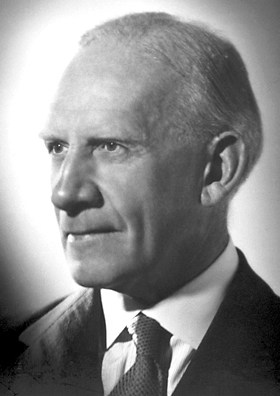
\includegraphics[width=\linewidth]{images/book3/robinson.jpg}
\end{minipage}\hfill
\begin{minipage}[t]{0.78\linewidth}
\vspace{0pt}
نشر روبرت روبنسون ووليام رابسون سلسلة تكوين الحلقة سنة 1935، في عمل يستهدف
تخليق الستيرويدات. وكانت إنجازات روبنسون الرئيسية بنى القلويدات وتخليقها،
ونال عنها جائزة نوبل في الكيمياء سنة 1947. وفي سنة 1950 صنع بيتر فيلاند وكارل ميشر
ثنائي الكيتون الثنائي الحلقة في مسألة هذا الفصل، الذي صار نقطة انطلاق شائعة لتخليق الستيرويدات 
والتربينات. (صورة شخصية: مؤلف مجهول، ملكية عامة؛ ويكيميديا كومنز.)
\end{minipage}
\end{history}

\begin{safety}{\ghs[5mm]{GHS02}\,\ghs[5mm]{GHS05}\,\ghs[5mm]{GHS06}\,\ghs[5mm]{GHS07}\,\ghs[5mm]{GHS08}\,\ghs[5mm]{GHS09}}
البوت-3-ين-2-ون قابل للاشتعال، وشديد السمية، وأكّال وخطر على البيئة المائية، ومسيل قوي للدموع؛ ولا يُتداول إلا
تحت ساحبة أبخرة. والهكس-2-ين حلقي-1-ون قابل للاشتعال وسام. والمركبات العضوية الليثيومية وكواشف غرينيار 
والكوبرات تتفاعل بعنف مع الماء وتُتداول تحت غاز خامل.
% ledger: ghs:MVK, ghs:cyclohexenone, ghs:MeMgBr
\end{safety}

\section{تمارين}

\begin{exercise}[$\star$]\label{exo:b2:conjugate-additions:1}
تنبأ \omterm{def:b2:conjugate-additions:addition-modes}{بالإضافة 1،2} أو 1،4 إلى الهكس-2-ين حلقي-1-ون من أجل: \ce{CH3MgBr}؛ \ce{(CH3)2CuLi}؛
\ce{C6H5SH} مع قليل من القاعدة؛ \ce{LiAlH4}.
\end{exercise}

\begin{exercise}[$\star$]\label{exo:b2:conjugate-additions:2}
صنّف إلى \omterm{def:b2:conjugate-additions:michael}{مانح مايكل} أو \omterm{def:b2:conjugate-additions:michael}{مستقبل مايكل}: البنتان-2،4-ديون، والبروبيننتريل \ce{CH2=CHCN}،
والنتروميثان، وبروبينوات الميثيل، وبروبانديوات ثنائي الإيثيل، والبوت-3-ين-2-ون.
\end{exercise}

\begin{exercise}[$\star$]\label{exo:b2:conjugate-additions:3}
اكتب تحضير ثنائي بيوتيل كوبرات الليثيوم من 1-بروموبيوتان والليثيوم ويوديد النحاس(I).
\end{exercise}

\begin{exercise}[$\star$]\label{exo:b2:conjugate-additions:4}
أعطِ ناتج بروبانديوات ثنائي الإيثيل مع البوت-3-ين-2-ون وكمية حفزية من إيثوكسيد
الصوديوم، ثم الناتج بعد الحلمهة والتسخين.
\end{exercise}

\begin{exercise}[$\star\star$]\label{exo:b2:conjugate-additions:5}
اقترح تحضيرًا للمركب 3-ميثيل هكسانون حلقي من الهكس-2-ين حلقي-1-ون، وفسّر لماذا يكون
بروميد ميثيل المغنيزيوم خيارًا رديئًا.
\end{exercise}

\begin{exercise}[$\star\star$]\label{exo:b2:conjugate-additions:6}
يُضاف الإيثانثيول إلى البوت-3-ين-2-ون مع أثر من ثلاثي إيثيل أمين. اكتب الآلية وقل لماذا
يُضاف الثيولات إضافة 1،4.
\end{exercise}

\begin{exercise}[$\star\star$]\label{exo:b2:conjugate-additions:7}
يعطي السيانيد مع الهكس-2-ين حلقي-1-ون، في درجة حرارة منخفضة ولأزمنة قصيرة، السيانوهيدرين؛ وفي درجة حرارة
أعلى ولأزمنة أطول، 3-أوكسو هكسان حلقي-1-كربونتريل. فسّر بالتحكم الحركي والترموديناميكي.
\end{exercise}

\begin{exercise}[$\star\star$]\label{exo:b2:conjugate-additions:8}
أعطِ ناتج \omterm{def:b2:conjugate-additions:robinson}{الإلحاق الحلقي لروبنسون} للمركب 2-ميثيل هكسان حلقي-1،3-ديون مع البوت-3-ين-2-ون، ثم ناتج
الهكسانون الحلقي مع البوت-3-ين-2-ون.
\end{exercise}

\begin{exercise}[$\star\star$]\label{exo:b2:conjugate-additions:9}
فكّك الهبتان-2،6-ديون إلى \omterm{def:b2:conjugate-additions:michael}{مانح مايكل} \omterm{def:b2:conjugate-additions:michael}{ومستقبل مايكل}، واقترح الظروف.
\end{exercise}

\begin{exercise}[$\star\star\star$]\label{exo:b2:conjugate-additions:10}
\omterm{def:b2:enolates-aldol:aldol}{الإضافة الألدولية} البسيطة تنعكس بسهولة في القاعدة؛ أما ناتج \omterm{def:b2:conjugate-additions:michael}{إضافة مايكل} لبروبانديوات ثنائي الإيثيل 
والبوت-3-ين-2-ون فلا. فسّر بالروابط المتكوّنة والمنكسرة وبحموضة الناتج.
\end{exercise}

\begin{exercise}[$\star\star\star$]\label{exo:b2:conjugate-additions:11}
يعطي بروبانديوات ثنائي الإيثيل مع مكافئين من بروبينوات الميثيل وقاعدة حفزية ناتجًا
لا تبقى فيه أي رابطة \ce{C-H} بين مجموعتي الإستر. ارسمه وفسّر.
\end{exercise}

\begin{exercise}[$\star\star\star$]\label{exo:b2:conjugate-additions:12}
يمكن أن يتفاعل 2-ميثيل هكسانون حلقي والبوت-3-ين-2-ون في \omterm{def:b2:conjugate-additions:robinson}{إلحاق حلقي لروبنسون} عبر أي من أيوني الإينولات.
ارسم الناتجين وقل أي الظروف تحابي الناتج الذي تقع فيه مجموعة الميثيل على كربون التحام
الحلقتين.
\end{exercise}

\section{مسألة: كيتون فيلاند--ميشر}

\begin{problem}[{مسألة نهاية الأسبوع --- المانح الحمضي، وناتج إضافة مايكل، والألدول الداخلي الجزيء 
ونزع الماء منه، والمركز الفراغي والموازنة الكتلية لتحضير}]
\label{pb:b2:conjugate-additions:1}
التحضير (معطيات تمرين): يتفاعل \qty{10.0}{g} من 2-ميثيل هكسان حلقي-1،3-ديون مع فائض طفيف
من البوت-3-ين-2-ون وقاعدة حفزية (\omterm{def:b2:conjugate-additions:michael}{إضافة مايكل})؛ ثم يُحلقن ثلاثي الكيتون \omterm{def:b2:amines:class}{بأمين
ثانوي} وحمض (\omterm{def:b2:enolates-aldol:aldol}{ألدول}، ونزع الماء). المردود الإجمالي: 70~\%. وللمركب الأم هكسان حلقي-1،3-ديون
$\mathrm pK_a = 5.3$ في الماء. والكتل المولية (\unit{g/mol}): C 12.011، H 1.008، O 15.999.
% ledger: pka:cyclohexanedione, aw:C, aw:H, aw:O, ghs:methylcyclohexanedione, ghs:MVK

\medskip
\noindent\textbf{الجزء الأول --- المانح.}
\begin{enumerate}
  \item ارسم 2-ميثيل هكسان حلقي-1،3-ديون وعلّم أكثر هيدروجيناته حموضة.
  \item لماذا يكون ذلك الهيدروجين أكثر حموضة بكثير من هيدروجينات $\alpha$ في الهكسانون الحلقي؟
  \item ارسم بنى الرنين الثلاث لأيون إينولاته.
  \item هل الهيدروكسيد أو الإيثوكسيد قوي بما يكفي لتكوين \omterm{def:b2:enolates-aldol:enolate}{أيون الإينولات} هذا كليًا؟ استعمل قيمة $\mathrm pK_a$.
  \item اكتب \omterm{def:b2:enolates-aldol:tautomerism}{إينول} الديون الذي يشمل C2، وقل لماذا لا تمنعه مجموعة الميثيل على C2
        من ذلك.
  \item هل \omterm{def:b2:enolates-aldol:enolate}{أيون الإينولات} هذا قاسٍ أم لين؟ وأي موقع من البوت-3-ين-2-ون سيهاجم؟
\end{enumerate}

\medskip
\noindent\textbf{الجزء الثاني --- ناتج \omterm{def:b2:conjugate-additions:michael}{إضافة مايكل}.}
\begin{enumerate}[resume]
  \item اكتب \omterm{def:b2:conjugate-additions:michael}{إضافة مايكل} وسمِّ ثلاثي الكيتون المتكوّن.
  \item لماذا لا تلزم إلا كمية حفزية من القاعدة؟
  \item لماذا تتكوّن الرابطة الجديدة عند C2 في الديون لا عند أكسجينه؟
  \item كم ذرة كربون رباعية في ثلاثي الكيتون؟
  \item حدّد علاقة 1،5-ثنائي الكربونيل في ثلاثي الكيتون.
  \item لماذا يُستعمل فائض طفيف من البوت-3-ين-2-ون، ولماذا طفيف فقط؟
\end{enumerate}

\medskip
\noindent\textbf{الجزء الثالث --- غلق الحلقة.}
\begin{enumerate}[resume]
  \item عدّد كربونات ثلاثي الكيتون التي تحمل هيدروجينات $\alpha$.
  \item أي أيون إينولات، مهاجمًا أي كربونيل، يغلق حلقة سداسية؟
  \item ما عمليات غلق الحلقة الأخرى التي يمكن أن تُجرَّب، ولماذا لا تعطي الناتج؟
  \item اكتب \omterm{def:b2:enolates-aldol:aldol}{الألدول} المتكوّن ونزع الماء الذي يليه.
  \item لماذا يكون نزع الماء سهلًا؟
  \item سمِّ المجموعات الوظيفية في كيتون فيلاند--ميشر.
\end{enumerate}

\medskip
\noindent\textbf{الجزء الرابع --- الكيمياء الفراغية والموازنة الكتلية.}
\begin{enumerate}[resume]
  \item أي كربون في الناتج مركز فراغي؟
  \item هل ناتج هذا التحضير نشط ضوئيًا؟ فسّر.
  \item احسب الكتل المولية للديون، وللبوت-3-ين-2-ون وللناتج
        \ce{C11H14O2}.
  \item اكتب المعادلة الإجمالية وتحقق منها بالصيغ.
  \item احسب كمية الديون المستعملة.
  \item اذكر كتلة كيتون فيلاند--ميشر الناتجة بمردود إجمالي 70~\%.
\end{enumerate}
\end{problem}
